\addcontentsline{toc}{subsubsection}{\strut \hspace{24mm} Spatial averaging}

\vspace{\baselineskip} 
\vspace{\baselineskip} 
\noindent {\bf Spatial averaging}

\opthead{PR3}{\ws}{H. L. Tolman}


The major drawback of the above GSE alleviation method is its potential impact
on model economy as discussed in relation to Eq.~(\ref{eq:ddif_4}) and in
\cite{tol:Waves01a,tol:OMOD02b}. For this reason, an alternative additional GSE alleviation
method has been developed for \ws.

This method which represents the default for \ws, replaces the
additional diffusion step (\ref{eq:d_bal_1}) with a separate fractional step
in which direct averaging of the field of energy densities for a given
spectral component is considered. The area around each grid point over which
the averaging is performed extends in the propagation ($\bs$) and normal
($\bn$) directions as

\begin{equation}
\pm \gamma_{a,s} \: \Delta c_g \: \Delta t \: \bs \:\:\: ,
\pm \gamma_{a,n} \: c_g \Delta \theta \: \Delta t \: \bn \:\:\: , \label{eq:GSE_avg}
\end{equation}

\noindent
where $\gamma_{a,s}$ and $\gamma_{a,n}$ are tunable constants, the default
value of which is set to 1.5. This averaging is illustrated in
Fig.~\ref{fig:GSE_1}. Note that these values may require some retuning for
practical applications, as discussed in \cite{tol:OMOD02b}. Appendix A of the
latter paper presents details of the averaging scheme, including conservation
considerations. Consistency with the \cite{art:BH87} approach furthermore
implies that $\gamma_{a,s}$ and $\gamma_{a,n}$ should vary with the spatial
grid resolution \citep[see][Appendix]{tol:OMOD08a}.

Note that this kind of averaging with dominant directions $\bs$ and $\bn$ is
similar to the \cite{art:BH87} diffusion method, that uses the same main
directions. The averaging method, however, never influences the time step,
because it is completely separated from the actual propagation. Moreover, if
explicit schemes are used with typically $c_g \Delta t / \Delta x < 1$, it is
obvious that the averaging over the area as defined in (\ref{eq:GSE_avg}) will
generally require information at directly neighboring spatial grid points
only, as in Fig.~\ref{fig:GSE_1}. Furthermore, this method does not require
high-latitude filtering.

\begin{figure} \begin{center}
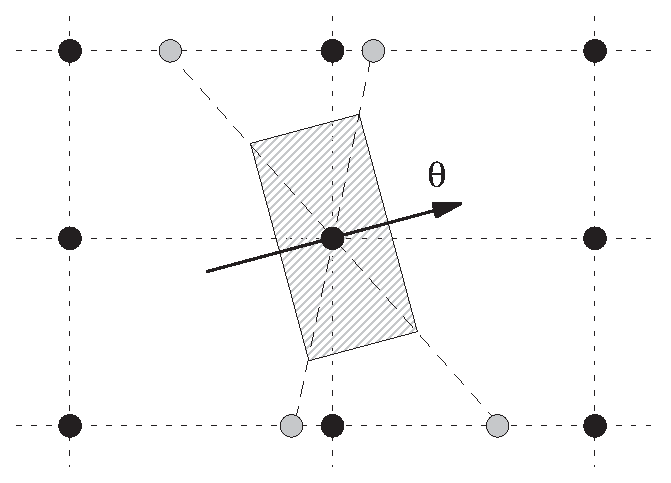
\epsfig{file=./num/GSE_1.eps,angle=0,width=2.2in}
\caption{Schematic of spatial averaging GSE alleviation technique. 
Solid circles and dotted lines represent the spatial grid. Hatched
area represent averaging area to be considered. Corner point values are
obtained from the central grid point and the gray points. The latter values
are obtained by interpolation from adjacent grid points
\citep[from][]{tol:OMOD02b}.}
\label{fig:GSE_1} \botline
\end{center}
\end{figure}

As is illustrated in \cite{tol:OMOD02b,tol:OMB02b}, this method gives
virtually identical results as the previous method, but does so at slightly
lower costs. For high-resolution applications, the averaging method may become
dramatically more economical.



Finally, the GSE can be alleviated somewhat by assuring that the discrete
spectral directions do not coincide with spatial grid lines. This can be
achieved by defining the first discrete direction $\theta_1$ as

% eq:theta1          First direction

\begin{equation}
\theta_1 = \alpha_\theta \: \Delta \theta \:\:\: , \label{eq:theta1}
\end{equation}

\noindent
where $-0.5 \leq \alpha_\theta \leq 0.5$ can be defined by the user. Note that
setting $\alpha \neq 0$ is beneficial to the first-order scheme, but has
negligible impact on the third-order scheme.
 
